% BEGIN LICENSE BLOCK
% Version: CMPL 1.1
%
% The contents of this file are subject to the Cisco-style Mozilla Public
% License Version 1.1 (the "License"); you may not use this file except
% in compliance with the License.  You may obtain a copy of the License
% at www.eclipse-clp.org/license.
% 
% Software distributed under the License is distributed on an "AS IS"
% basis, WITHOUT WARRANTY OF ANY KIND, either express or implied.  See
% the License for the specific language governing rights and limitations
% under the License. 
% 
% The Original Code is  The ECLiPSe Constraint Logic Programming System. 
% The Initial Developer of the Original Code is  Cisco Systems, Inc. 
% Portions created by the Initial Developer are
% Copyright (C) 2006 Cisco Systems, Inc.  All Rights Reserved.
% 
% Contributor(s): 
% 
% END LICENSE BLOCK

%----------------------------------------------------------------------
\chapter{Implementing Constraints}
\label{chapimpl}
%HEVEA\cutdef[1]{section}
%----------------------------------------------------------------------

This chapter describes how to use \eclipse{}'s advanced control
\index{implementing constraints}
facilities for implementing constraints.
Note that the Generalised Propagation library lib(propia) and
the Constraint Handling Rules library lib(ech) provide other,
higher-level ways to implement constraints. Those are more
suited for prototyping, while this chapter introduces those low-level
primitives that are actually used in the implementation of the various
\eclipse{} constraint solvers.


%----------------------------------------------------------------------
\section{What is a Constraint in Logic Programming?}
%----------------------------------------------------------------------

Constraints fit very naturally into the Logic Programming paradigm.
Declaratively, a constraint is just the same as any other predicate.
Indeed, in \eclipse{}, ``constraints'' are not a particular
programming language construct, constraints are just a conceptual notion.

Consider the following standard Prolog query:
\begin{quote}\begin{verbatim}
?- member(X, [5,7,3,4]), X =< 4.
\end{verbatim}\end{quote}
This will succeed with X = 3 after some search.
In this example, both the member/2 goal and the inequality goal could
be considered `constraints on X' because they both restrict the
possible values for X. Usually, however, member/2 would not be considered
a ``constraint'' because of its backtracking (search) behaviour:
\begin{quote}\begin{verbatim}
?- member(X, [5, 7, 3, 4]).
X = 5
More (0.00s cpu)
X = 7
More (0.04s cpu)
\end{verbatim}\end{quote}
Also, the standard Prolog inequality would not be considered a ``constraint'',
because if invoked on its own it will raise an error:
\begin{quote}\begin{verbatim}
?- X =< 4.
instantiation fault in X =< 4
\end{verbatim}\end{quote}
\index{constraint}
In the following, we will call a predicate a {\bf constraint} only if it
\begin{itemize}
\item behaves deterministically
\item somehow actively enforces its declarative meaning
\end{itemize}


%----------------------------------------------------------------------
\section{Background: Constraint Satisfaction Problems}
\index{constraint satisfaction problem}
\index{CSP}
\label{csp}
%----------------------------------------------------------------------

There is a large body of scientific work and literature about
Constraint Satisfaction Problems, or CSPs.
CSPs are a restricted class of constraint problems with the
following properties
\enableunderscores
\begin{itemize}
\item there is a fixed set of variables $X_1, ..., X_n$
\item every variable $X_i$ has a finite domain $D_i$ of values that the variable
        is allowed to take. In general, this can be an arbitrary, unordered
        domain.
\item usually one considers only binary (2-variable) constraints $c_{ij}(X_i,X_j)$.
        Every constraint is simply defined as a set of pairs of consistent values.
\item the problem is to find a valuation (labeling) of the variables such
        that all the constraints are satisfied.
\end{itemize}
\disableunderscores
The restriction to binary constraints is not really limiting since every CSP
can be transformed into a binary CSP. However, this is often not necessary
since many algorithms can be generalised to n-ary constraints.

A CSP network is the graph formed by considering the variables as nodes
and the constraints as arcs between them.
In such a network, several levels of consistency can be defined:
\index{node consistency}
\index{arc consistency}
\index{path consistency}
\enableunderscores
\begin{description}
\item[Node consistency] $\forall{v \in D_i} : c_i(v)$
        (not very interesting).  It means that
	all unary constraints are reflected in the domains
\item[Arc consistency] $\forall{v \in D_i}\ \exists{w \in D_j} : c_{ij}(v,w)$
	(most practically relevant).
	It means that for every value in the domain of one
	variable, there is a compatible value in the domain of the
	other variable in the constraint.  In practice, constraints
	are symmetric, so the reverse property also holds.
\item[Path consistency] $\forall{v \in D_i}\ \forall{w \in D_j}\ \exists{u \in D_k} : c_{ik}(v,u), c_{kj}(u,w)$
        (usually too expensive). One can show that this property extends to
	whole paths, i.e.\ on any path of constraints between variables i and j 
	the variables have domain values which are compatible with any
	domain values for i and j.
\end{description}
\disableunderscores
Note that neither of these conditions is sufficient for the
problem to be satisfiable. It is still necessary to search for solutions.
Computing networks with these consistency levels can however be a useful
intermediate step to finding a solution to the CSP.

Consequently, a complete CSP solver needs the following design decisions:
\begin{itemize}
\item what level of consistency do we want to employ?
\item at what time during search do we want to (re)establish this consistency?
\item what algorithm do we use to establish this consistency?
\end{itemize}
In practice, the most relevant consistency level is arc-consistency.
Consequently, a number of algorithms have been proposed for the
purpose of establishing arc-consistency. The algorithms used in \eclipse{}
\index{AC-3}
are mostly variants of AC-3 \cite{mackworth77}
\index{AC-5}
and AC-5 \cite{vanhentenryck92generic}.

\ignore{
procedure REVISE(Vi,Vj)
    DELETE <- false;
    for each X in Di do
        if there is no such Y in Dj such that (X,Y) is consistent,
        then
            delete X from Di;
            DELETE <- true;
        endif;
    endfor;
    return DELETE;
    end REVISE

procedure AC-3
    Q <- {(Vi,Vj) in arcs(G),i#j};
    while not Q empty
        select and delete any arc (Vk,Vm) from Q;
        if REVISE(Vk,Vm) then
            Q <- Q union {(Vi,Vk) such that (Vi,Vk) in arcs(G),i#k,i#m}
        endif
    endwhile
    end AC-3
}


%----------------------------------------------------------------------
\section{Constraint Behaviours}
\index{behaviour of a constraint}
%----------------------------------------------------------------------

As opposed to the theoretical CSP framework sketched in the previous section,
in \eclipse{} we usually deal with more heterogeneous situation.
We want to allow the integration of very different constraints,
and we want to achieve a separation of constraint propagation and search.
Therefore, we are not interested in an overall problem solving algorithm
which controls search and constraint propagation globally for the whole
problem and all constraints.
We prefer to view the constraint solving process as in figure \ref{figclpexec}:
the search process is controlled by an algorithmic program,
while constraint propagation is performed by data-driven agents which
do local (again algorithmic) computations on one or several constraints.
\begin{figure}
\begin{center}
\resizebox{0.4\textwidth}{!}{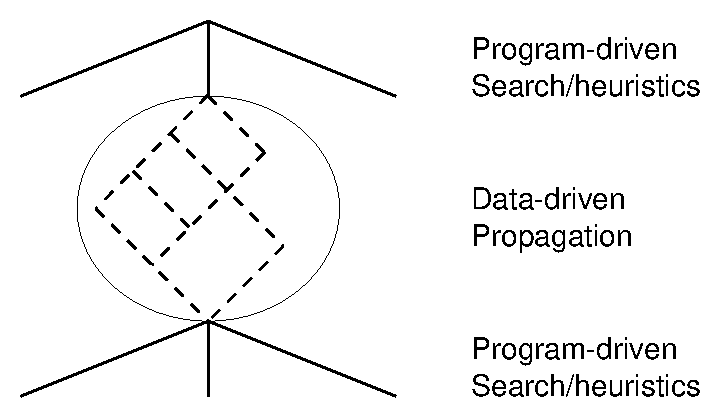
\includegraphics{clpexec.eps}}
\end{center}
\caption{Control during Constraint Solving}
\label{figclpexec}
\end{figure}
Individual constraints can then be implemented with different behaviours,
and freely mixed within a single computation.
Constraint behaviours can essentially be characterised by
\index{trigger condition}
\begin{itemize}
\item their triggering condition ({\bf when} are they executed)
\item the action they perform when triggered ({\bf what} do they do)
\end{itemize}
Let us now look at examples of different constraint behaviours.

\subsection{Consistency Check}
\index{consistency check}
The \verb.=<./2 predicate, whose standard Prolog version raises an error
when invoked with uninstantiated variable, is also implemented by the
{\bf suspend} library. Both implementations
have the same declarative meaning, but the {\bf suspend} version can
be considered to be a proper constraint.
It implements a {\bf passive test}, i.e.\
it simply delays until both arguments are numbers, and then succeeds or fails:
\begin{quote}\begin{verbatim}
?- suspend : (X =< 4).
X = X
There is 1 delayed goal.
Yes (0.00s cpu)

?- suspend : (X =< 4), X = 2.
X = 2
Yes (0.00s cpu)

?- suspend : (X =< 4), X = 5.
No (0.00s cpu)
\end{verbatim}\end{quote}

\subsection{Forward Checking}
\index{forward checking}
Often a constraint can already do useful work before all its arguments
are instantiated. In particular, this is the case when we are working
with domain variables. Consider {\bf ic}'s disequality constraint \verb.#\=.  :
Even when only one side is instantiated, it can already remove this value
from the domain of the other (still uninstantiated) side:
\begin{quote}\begin{verbatim}
?- X :: 1 .. 5,
   X #\= 3.
X = X{[1, 2, 4, 5]}
Yes (0.00s cpu)
\end{verbatim}\end{quote}
If both sides are uninstantiated, the constraint cannot do anything useful.
It therefore waits (delays) until one side becomes instantiated,
but then wakes up and acts as before.
This behaviour is sometimes called forward checking \cite{VanHentenryck}:
\begin{quote}\begin{verbatim}
?- [X,Y] :: 1 .. 5,
   X #\= Y.        % delays
X = X{1 .. 5}
Y = Y{1 .. 5}
There is 1 delayed goal.
Yes (0.00s cpu)

?- X :: 1 .. 5,
   X #\= Y,         % delays
   Y = 3.           % wakes
X = X{[1, 2, 4, 5]}
Y = 3
Yes (0.01s cpu)
\end{verbatim}\end{quote}

\subsection{Domain (Arc) Consistency}
\index{arc consistency}
\index{domain consistency}
For many constraints, even more eager behaviour is possible.
For example, {\bf ic}'s inequality constraints performs {\bf domain updates} as
soon as possible, even when one or both arguments are still variables:
\begin{quote}\begin{verbatim}
?- [X, Y] :: 1 .. 5, X #< Y.
X = X{1 .. 4}
Y = Y{2 .. 5}
There is 1 delayed goal.
Yes (0.00s cpu)

?- [X, Y] :: 1 .. 5, X #< Y, X #> 2.
Y = Y{[4, 5]}
X = X{[3, 4]}
There is 1 delayed goal.
Yes (0.00s cpu)
\end{verbatim}\end{quote}
Inconsistent values are removed form the domains as soon as possible.
This behaviour corresponds to {\bf arc consistency} as discussed in
section \ref{csp}.

\subsection{Bounds Consistency}
\index{bounds consistency}
Note however that not all {\bf ic} constraints maintain full domain
arc consistency.  For performance reasons, 
the \verb.#=. constraint only maintains bounds consistency, which is
weaker, as illustrated by the following example:
\begin{quote}\begin{verbatim}
?- [X, Y] :: 1 .. 5, X #= Y + 1, X #\= 3.
Y = Y{1 .. 4}
X = X{[2, 4, 5]}
There is 1 delayed goal.
Yes (0.00s cpu)
\end{verbatim}\end{quote}
Here, the value 2 for Y was not removed even though it is not arc consistent
(there is no value for X which is compatible with it).

\index{incompleteness of propagation}
It is important to understand that this kind of propagation incompleteness
does not affect correctness: the constraint will simply detect the
inconsistency later, when its arguments have become more instantiated.
In terms of the search tree, this means that a branch will not be pruned
as early as possible, and extra time might be spent searching.


\quickref{Typical Constraint Behaviours}{
\begin{description}
\item[Consistency Checking] 
        wait until all variables instantiated, then check
\item[Forward Checking] 
        wait until one variable left, then compute consequences
\item[Domain (Arc) Consistency] 
        wait until a domain changes, then compute consequences for other domains
\item[Bounds Consistency] 
        wait until a domain bound changes, then compute consequences for other bounds
\end{description}
}


\ignore{
\subsection{The Resolvent}
\index{resolvent}
The term {\bf resolvent} originates from Logic Programming.
It is the set of all goals that need to be satisfied.
The computation typically starts with a top-level goal,
then gets successively transformed (by substituting goals that
match a clause head with an instance of the clause body, ie.\ a
sequence of sub-goals),
and eventually terminates with one of the trivial goals
{\bf true} or {\bf fail}.
For example, given the program
\begin{quote}\begin{verbatim}
p :- q,r.
q.
r :- q.
\end{verbatim}\end{quote}
and the goal p, the resolvent goes through the following states
before the goal is proven and the computation terminates:
\begin{quote}\begin{verbatim}
p ----> q,r ----> r ----> q ----> {}
\end{verbatim}\end{quote}

\index{Prolog}
While in Prolog the resolvent is always processed from left to right,
the resolvent in {\eclipse} is more structured, and can be manipulated
in a much more flexible way.
This is achieved by two basic mechanisms, {\bf suspension}
and {\bf priorities}.

\index{suspended goal}
{\bf Suspended} goals form the part of the resolvent which is
currently not being considered. This is typically done when we
know that we cannot currently infer any interesting information from them.

\index{priority}
The remaining goals are ordered according to their {\bf priority}.
At any time, the system attempts to solve the most urgent subgoal first.
{\eclipse} currently supports a fixed range of 12 different priorities,
priority 1 being the most urgent and 12 the least urgent.

Figure \ref{figresolv} shows the structure of the resolvent.
When a toplevel goal is launched, it has priority 12 and is the only
member of the resolvent. As execution proceeds, active goals may be
suspended, and suspended goals may be woken and scheduled with a
particular priority.
\begin{figure}
% picture has been made with xfig and exported as encapsulated postscript
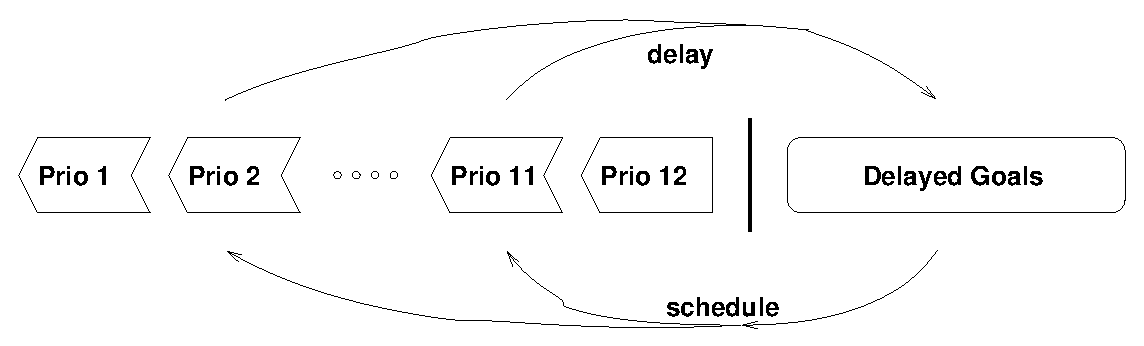
\includegraphics{resolv.eps}
\caption{Structure of the resolvent}
\label{figresolv}
\end{figure}
}



%----------------------------------------------------------------------
\section{Programming Basic Behaviours}
%----------------------------------------------------------------------

As an example, we will look at creating constraint versions of the
following predicate.
It defines a relationship between containers of type 1, 2 or 3,
and their capacity:
\begin{code}
capacity(1, N) :- N>=0.0, N=<350.0.
capacity(2, N) :- N>=0.0, N=<180.0.
capacity(3, N) :- N>=0.0, N=<50.0.
\end{code}
This definition gives the intended declarative meaning,
but does not behave as a constraint:
{\tt capacity(3, C)} will raise an error, and
{\tt capacity(Type, 30.5)} will generate several solutions nondeterministically.
Only calls like {\tt capacity(3, 27.1)} will act correctly as a test.


\subsection{Consistency Check}
\index{consistency check}

To program the passive consistency check behaviour, we need to wait until
both arguments of the predicate are instantiated.
This can be achieved by adding an \eclipse{} {\bf delay clause}:
\begin{code}
delay capacity(T,N) if var(T);var(N).
capacity(1, N) :- N>=0.0, N=<350.0.
capacity(2, N) :- N>=0.0, N=<180.0.
capacity(3, N) :- N>=0.0, N=<50.0.
\end{code}
The delay clause specifies that any call to capacity/2 will delay as long
as one of the arguments is a variable. When the variables become instantiated
later, execution will be resumed automatically, and 
the instantiations will be checked for satisfying the constraint.


\subsection{Forward Checking}
\index{forward checking}

For Forward Checking, we will assume that we have interval domain variables,
as provided by the {\bf ic} library (without domain variables, there would
not be much interesting propagation to be done).

Here is one implementation of a forward checking version:
\begin{code}
:- lib(ic).
delay capacity(T, N) if var(T), var(N).
capacity(T, N) :- nonvar(N), !,
        N >= 0,
        ( N =< 50.0 -> T :: [1,2,3]
        ; N =< 180.0 -> T :: [1,2]
        ; N =< 350.0 -> T = 1
        ; fail
        ).
capacity(1, N) :- N\$>=0.0, N\$=<350.0.
capacity(2, N) :- N\$>=0.0, N\$=<180.0.
capacity(3, N) :- N\$>=0.0, N\$=<50.0.
\end{code}
Note that the delay clause now only lets goals delay when both
arguments are variables. As soon as one is instantiated, the
goal wakes up and, depending on which is the instantiated argument,
either the first, or one of the last three clauses is executed.
Some examples of the behaviour:
\begin{quote}\begin{verbatim}
?- capacity(T, C).
There is 1 delayed goal.
Yes (0.00s cpu)

?- capacity(3, C).
C = C{0.0 .. 50.0}
Yes (0.00s cpu)

?- capacity(T, C), C = 100.
T = T{[1, 2]}
C = 100
Yes (0.00s cpu)
\end{verbatim}\end{quote}

A disadvantage of the above implementation is that when the predicate wakes
up, it can be either because T was instantiated, or because C was
instantiated. An extra check ({\tt nonvar(N)}) is needed to distinguish the two cases.
Alternatively, we could have created two agents (delayed goals), each one
specialised for one of these cases:
\begin{code}
capacity(T, N) :-
        capacity_forward(T, N),
        capacity_backward(T, N).

delay capacity_forward(T, _N) if var(T).
capacity_forward(1, N) :- N\$>=0.0, N\$=<350.0.
capacity_forward(2, N) :- N\$>=0.0, N\$=<180.0.
capacity_forward(3, N) :- N\$>=0.0, N\$=<50.0.

delay capacity_backward(_T, N) if var(N).
capacity_backward(T, N) :-
        N >= 0,
        ( N =< 50.0 -> T :: [1,2,3]
        ; N =< 180.0 -> T :: [1,2]
        ; N =< 350.0 -> T = 1
        ; fail
        ).
\end{code}
Unfortunately, there is a drawback to this implementation as well:
once one of the two delayed goals has done its work, all the constraint's
information has been incorporated into the remaining variable's domain.
However, the other delayed goal is still waiting, and will eventually
wake up when the remaining variable gets instantiated as well, at which time
it will then do a redundant check.

The choice between having one or several agents for a constraint is a
choice we will face every time we implement a constraint.



%----------------------------------------------------------------------
\section{Basic Suspension Facility}
%----------------------------------------------------------------------

For the more complex constraint behaviours (beyond those waiting for
instantiations), we need to employ lower-level primitives of the \eclipse{}
kernel (suspensions and priorities).
\index{suspension}
\index{priority}
If we want to add a new constraint to an existing solver, we also
need to use the lower-level interface that the particular solver
provides.

Apart from the delay clauses used above,
\eclipse{} also provides a more powerful (though less declarative) way of
causing a goal to delay.
The following is another implementation of the constraint checking behaviour,
this time using the suspend/3 built-in predicate to create a delayed goal for
\index{suspend/3}
capacity/2:
\begin{code}
capacity(T,N) :- (var(T);var(N)), !,
        suspend(capacity(T,N), 0, [T,N]->inst).
capacity(1, N) :- N>=0.0, N=<350.0.
capacity(2, N) :- N>=0.0, N=<180.0.
capacity(3, N) :- N>=0.0, N=<50.0.
\end{code}
\quickref{The Basic Suspension Facilities}{
\begin{description}
\item[{\bf suspend(Goal, Priority, Triggers)}] 
	\index{suspend/3}
        Creates Goal as a delayed goal with a given waking priority and
        triggering conditions.
        Triggers is a list of Variables->Conditions terms, specifying
        under which conditions the goal will be woken up.
        The priority specifies with which priority the goal will be scheduled
        after it has been triggered.
        A priority of 0 selects the default for the predicate.
        Otherwise, valid priorities range are from
        1 (most urgent, reserved for debugging purposes) to 12 (least urgent).
\end{description}
Some valid triggers:
\index{trigger condition}
\begin{description}
\item[X->inst] wake when the variable becomes instantiated (most specific)
\item[X->constrained] wake when the variable becomes constrained somehow
        (most general)
\item[X->ic:min] wake when the lower bound of an ic-variable changes
\item[X->ic:max] wake when the upper bound of an ic-variable changes
\item[X->ic:hole] wake an internal domain value gets removed
\end{description}
}


\section{A Bounds-Consistent IC constraint}

To show the basic ideas, we will simply reimplement a constraint that
already exists in the {\bf ic} solver, the inequality constraint.
We want a constraint ge/2 that takes two {\bf ic} variables (or numbers)
and constrains the first to be greater or equal to the second.

\index{bounds consistency}
The behaviour should be to maintain bounds-consistency:
If we have a goal {\tt ge(X,Y)}, where the domain of \verb/X is X{1..5}/ and
the domain of \verb/Y is Y{3..7}/, we would like the domains to be updated such
that the upper bound of Y gets reduced to 5, and the lower bound of X
gets increased to 3. The following code achieves this:
\begin{code}
ge(X, Y) :-
        get_bounds(X, _, XH),
        get_bounds(Y, YL, _),
        ( var(X),var(Y) ->
            suspend(ge(X,Y), 0, [X->ic:max, Y->ic:min])
        ;
            true
        ),
        X #>= YL,    % impose new bounds
        Y #=< XH.
\end{code}
We have used a single primitive from the low-level interface of the
{\bf ic} library:  {\bf get_bounds/3}, which extracts the current
domain bounds from a variable.  Further, we have used the information
that the library implements trigger conditions called {\bf min}
and {\bf max}, which cause a goal to wake up when the lower/upper
bound on an {\bf ic} variable changes.

Note that we suspend a new instance of the {\tt ge(X,Y)} goal {\em before}
we impose the new bounds on the variables. This is important when the
constraint is to be used together with other constraints of higher
priority: imposing a bound may immediately wake and execute such
a higher-priority constraint. The higher-priority constraint may then
in turn change one of the bounds that ought to wake ge/2 again.
This only works if ge/2 has already been (re-)suspended at that time.


\section{Using a Demon}
\index{demon}
Every time the relevant variable bounds change, the delayed ge/2 goal
wakes up and (as long as there are still two variables) a new,
identical goal gets delayed.
To better support this situation, {\eclipse} provides a special type
of predicate, called a {\bf demon}.
A predicate is turned into a
\index{demon}
demon by annotating it with a
\bipref{demon/1}{../bips/kernel/database/demon-1.html}
declaration.
A demon goal differs from a normal goal only in its behaviour on
waking. While a normal goal disappears from the resolvent when it is
woken, the demon remains in the resolvent.
Declaratively, this corresponds to an implicit recursive call in
the body of each demon clause.
Or, in other words, the demon goal forks into one goal that remains in the
suspended part of the resolvent, and an identical one
that gets scheduled for execution.

With a demon, our above example can be done more
efficiently. One complication arises, however. Since the goal
implicitly re-suspends, it now has to be explicitly killed when
it is no longer needed. The easiest way to achieve this is to
let it have a handle to itself (its `suspension') in one of its arguments.
This can then be used to kill the suspension when required:
\begin{code}
ge(X, Y) :-
        suspend(ge(X,Y,MySusp), 0, [X->ic:max, Y->ic:min], MySusp),
        ge(X, Y, MySusp).

:- demon ge/3.
ge(X, Y, MySusp) :-
        get_bounds(X, _, XH),
        get_bounds(Y, YL, _),
        ( var(X),var(Y) ->
            true     % implicitly re-suspend
        ;
            kill_suspension(MySusp)
        ),
        X #>= YL,    % impose new bounds
        Y #=< XH.
\end{code}
We have used the new primitives suspend/4 and kill_suspension/1.


%----------------------------------------------------------------------
%\section{Constraints with many variables}
%----------------------------------------------------------------------

%----------------------------------------------------------------------
\section{Exercises}
%----------------------------------------------------------------------

\begin{enumerate}

\item Implement a constraint atmost/3 
\begin{quote}\begin{verbatim}
atmost(+N, +List, +V)
\end{verbatim}\end{quote}
   which takes an integer N, an integer V and a list List
   containing integers or integer domain variables.

   Meaning: at most N elements of List have value V.

   Behaviour: Fail as soon as too many list elements are
   instantiated to value V.
   This requires only basic suspension facilities, no domain
   information needs to be taken into account.

   Tests are provided in the file {\tt atmost.tst}.
   You can test your constraint by loading the library {\tt lib(test_util)}
   and then calling {\tt test(atmost)}.


\item Implement a constraint offset/3

\begin{quote}\begin{verbatim}
offset(?X,+Const,?Y)
\end{verbatim}\end{quote}
which is declaratively like
\begin{quote}\begin{verbatim}
offset(X,Const,Y) :- Y #= X+Const.
\end{verbatim}\end{quote}
  but maintains domain-arc-consistency (i.e. propagates
  "holes", while the above definition only maintains
  bounds-consistency).

  Use suspension built-ins and domain-access primitives
  from the ic_kernel module.
  Use not_unify/2 to test whether a value is outside
  a variable's domain.

   Tests are provided in the file {\tt offset.tst}.
   You can test your constraint by loading the library {\tt lib(test_util)}.
   and then calling {\tt test(offset)}.

\end{enumerate}

%HEVEA\cutend
